% !TEX encoding = UTF-8 Unicode
% !TEX root = ../Rapport/rapport.tex

\section{Branch and bound}

\subsection{Principe général du branch\&bound}
La méthode du branch and bound consiste à énumérer les solutions d'un problème sous forme d'arbre binaire et à conserver à chaque pas la meilleure solution réalisable. Certaines branches de l'arbre ne sont pas évaluée lorsqu'elles donnent de moins bonnes solutions que la meilleure solution courante. Une méthode de séparation est appliquée à chaque nœud de l'arbre pour le partitionner en deux sous-problèmes et ainsi générer ses fils. Une méthode d'évaluation, quant à elle, sert à déterminer la solution optimale associée à un nœud de l'arbre.

\subsection{Méthode de séparation}
La méthode de séparation est utilisée pour séparer le problème en plusieurs sous-problèmes qui forment une partition de l'ensemble des solutions initiales. Les sous-problèmes générés sont les fils dans l'arbre du problème de départ.


\subsection{Méthode d'évaluation}
La méthode d'évaluation, quant à elle, est utilisée pour déterminer la solution optimale associée à un nœud de l'arbre.


\subsection{Stratégie de parcours}
Enfin, la stratégie de parcours de l'arbre consiste à générer les nœuds en largeur ou en profondeur.


\subsection{Solution initiale du voyageur de commerce}


\subsubsection{Chaine de poids le plus faible}
\begin{figure}[H]
	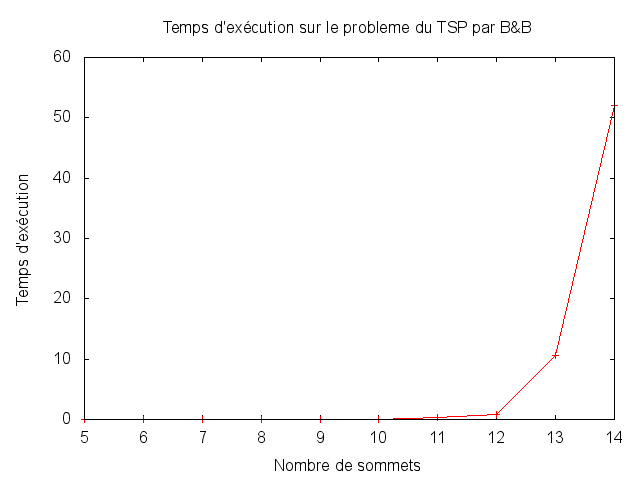
\includegraphics[width=\linewidth]{../pratique/branch_and_bound_dev/tsp_bb.png}
\end{figure}

\subsubsection{voisinage 2-opt}

\subsubsection{voisinage 3-opt}


\subsection{Comparaisons}


\subsection{Algorithme $\frac{3}{2}$ approché}



\section{Comparaison du Branch\&Bound et de la programmation dynamique sur l'exemple du TSP}


\begin{figure}[H]
	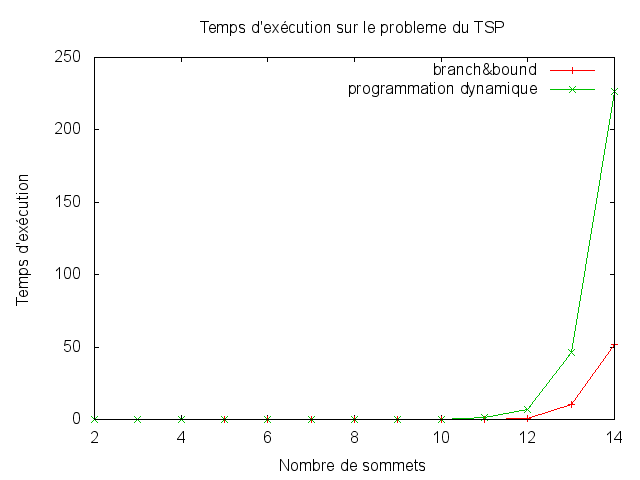
\includegraphics[width=\linewidth]{../pratique/comp.png}
\end{figure}


